\documentclass[journal]{IEEEtran}
\usepackage{cite}
\usepackage{amsmath,amssymb}
\usepackage{graphicx}
\usepackage{booktabs}
\usepackage[hidelinks]{hyperref}
\graphicspath{{../figures/}}
% generated by paper/make_figures.py -- do not edit
\newcommand{\sercsizero}{$0.184$}
\newcommand{\sercsifour}{$8.0\mathrm{e}{-2}$}
\newcommand{\sercsiseven}{$2.2\mathrm{e}{-2}$}
\newcommand{\sercsiten}{$1.3\mathrm{e}{-3}$}
\newcommand{\sercsitwelve}{$4.3\mathrm{e}{-5}$}
\newcommand{\sercsithirteen}{$5.2\mathrm{e}{-6}$}
\newcommand{\sercsifourteen}{$2.2\mathrm{e}{-7}$}
\newcommand{\sercsififteen}{$<2.1\mathrm{e}{-8}$}
\newcommand{\sercsiseventeen}{$<2.1\mathrm{e}{-8}$}
\newcommand{\serlszero}{$0.189$}
\newcommand{\serlsfour}{$8.3\mathrm{e}{-2}$}
\newcommand{\serlsseven}{$2.4\mathrm{e}{-2}$}
\newcommand{\serlsten}{$1.5\mathrm{e}{-3}$}
\newcommand{\serlstwelve}{$5.7\mathrm{e}{-5}$}
\newcommand{\serlsthirteen}{$6.4\mathrm{e}{-6}$}
\newcommand{\serlsfourteen}{$2.8\mathrm{e}{-7}$}
\newcommand{\serlsfifteen}{$<2.1\mathrm{e}{-7}$}
\newcommand{\serlsseventeen}{$<2.1\mathrm{e}{-7}$}
\newcommand{\servnetzero}{$0.210$}
\newcommand{\servnetfour}{$0.101$}
\newcommand{\servnetseven}{$3.2\mathrm{e}{-2}$}
\newcommand{\servnetten}{$3.3\mathrm{e}{-3}$}
\newcommand{\servnettwelve}{$5.6\mathrm{e}{-4}$}
\newcommand{\servnetthirteen}{$2.1\mathrm{e}{-4}$}
\newcommand{\servnetfourteen}{$1.2\mathrm{e}{-5}$}
\newcommand{\servnetfifteen}{$6.1\mathrm{e}{-5}$}
\newcommand{\servnetseventeen}{$2.0\mathrm{e}{-4}$}
\newcommand{\servnetfivezero}{$0.191$}
\newcommand{\servnetfivefour}{$8.4\mathrm{e}{-2}$}
\newcommand{\servnetfiveseven}{$2.5\mathrm{e}{-2}$}
\newcommand{\servnetfiveten}{$1.8\mathrm{e}{-3}$}
\newcommand{\servnetfivetwelve}{$9.9\mathrm{e}{-5}$}
\newcommand{\servnetfivethirteen}{$2.1\mathrm{e}{-5}$}
\newcommand{\servnetfivefourteen}{$5.6\mathrm{e}{-6}$}
\newcommand{\servnetfivefifteen}{$5.6\mathrm{e}{-6}$}
\newcommand{\servnetfiveseventeen}{$<4.2\mathrm{e}{-6}$}
\newcommand{\seraffinezero}{$0.191$}
\newcommand{\seraffinefour}{$8.5\mathrm{e}{-2}$}
\newcommand{\seraffineseven}{$2.7\mathrm{e}{-2}$}
\newcommand{\seraffineten}{$1.6\mathrm{e}{-3}$}
\newcommand{\seraffinetwelve}{$8.2\mathrm{e}{-5}$}
\newcommand{\seraffinethirteen}{$1.1\mathrm{e}{-5}$}
\newcommand{\seraffinefourteen}{$5.6\mathrm{e}{-6}$}
\newcommand{\seraffinefifteen}{$<4.2\mathrm{e}{-6}$}
\newcommand{\seraffineseventeen}{$<4.2\mathrm{e}{-6}$}
\newcommand{\sercsitwentyfivezero}{$0.192$}
\newcommand{\sercsitwentyfivefour}{$9.4\mathrm{e}{-2}$}
\newcommand{\sercsitwentyfiveseven}{$3.8\mathrm{e}{-2}$}
\newcommand{\sercsitwentyfiveten}{$9.8\mathrm{e}{-3}$}
\newcommand{\sercsitwentyfivetwelve}{$3.4\mathrm{e}{-3}$}
\newcommand{\sercsitwentyfivethirteen}{$2.0\mathrm{e}{-3}$}
\newcommand{\sercsitwentyfivefourteen}{$1.3\mathrm{e}{-3}$}
\newcommand{\sercsitwentyfivefifteen}{$8.5\mathrm{e}{-4}$}
\newcommand{\sercsitwentyfiveseventeen}{--}
\newcommand{\sertransformerzero}{$0.222$}
\newcommand{\sertransformerfour}{$0.104$}
\newcommand{\sertransformerseven}{$4.0\mathrm{e}{-2}$}
\newcommand{\sertransformerten}{$5.4\mathrm{e}{-3}$}
\newcommand{\sertransformertwelve}{$5.2\mathrm{e}{-4}$}
\newcommand{\sertransformerthirteen}{$1.4\mathrm{e}{-4}$}
\newcommand{\sertransformerfourteen}{$6.0\mathrm{e}{-5}$}
\newcommand{\sertransformerfifteen}{$1.5\mathrm{e}{-5}$}
\newcommand{\sertransformerseventeen}{$<4.2\mathrm{e}{-6}$}


\begin{document}

\title{ViterbiNet Revisited: A Matched-Information\\ Classical Baseline for Learned Trellis Detection}

\author{Gil~Zukerman%
\thanks{G. Zukerman is with the School of Electrical Engineering, Tel Aviv University, Tel Aviv 6997801, Israel (e-mail: gilzukerman@mail.tau.ac.il).}}

\markboth{IEEE Communications Letters}{ViterbiNet Revisited}

\maketitle

\begin{abstract}
ViterbiNet replaces the Viterbi algorithm's channel-dependent branch metric with a small neural network trained from pilots and adapted online on decoded words. Prior evaluations reported performance approaching Viterbi with perfect channel state information (CSI), and gains over uncertain or stale CSI. We add a matched baseline: a Viterbi detector that uses the same pilots (one word in 25) and the same code-based acceptance rule, applied to its own decisions, and estimates its four taps by least squares. On a coded BPSK channel with COST~2100 taps, this LS-Viterbi receiver has the lowest point-estimate SER of all no-CSI receivers from 0 to 14~dB. On shared draws it is significantly better than ViterbiNet with 5 adaptation updates, the best configuration here, at 1, 6, 7, and 9--12~dB and never significantly worse; 13--14~dB is not resolved. It stays within about 3--30\% of the perfect-CSI SER, consistent with a predicted 0.13~dB loss. Under an implementable, ground-truth-free adaptation gate, LS-Viterbi keeps the lowest point-estimate SER at the three SNRs tested. The default 200 Adam updates per word overfit: 5 give a lower SER at every SNR with 40 times fewer updates. A 32-parameter affine metric, the exact form of the Gaussian log-likelihood, matches the 7,002-parameter network. Only LS-Viterbi and ViterbiNet with 5 updates fit the measured detection-plus-adaptation time within a word on one CPU thread. In this experiment, the tested learned receivers show no established advantage over a classical receiver given the same information.
\end{abstract}

\begin{IEEEkeywords}
Deep learning, symbol detection, Viterbi algorithm, channel estimation, intersymbol interference, model-based deep learning.
\end{IEEEkeywords}

\section{Introduction}
\IEEEPARstart{M}{odel-based} deep learning keeps the structure of a classical algorithm and learns only the parts that depend on an unknown model~\cite{shlezinger2023mbdl}. ViterbiNet~\cite{shlezinger2020viterbinet} is a representative example for sequence detection over channels with memory: the Viterbi trellis~\cite{forney1973viterbi,forney1972mlse} is kept, and a small fully connected network maps each received sample to the likelihoods of the channel states. The network is trained on pilots and adapted online on decoded words that a Reed--Solomon (RS) code accepts, which lets the receiver follow a time-varying channel without new pilots. Later work added meta-learning to speed up that adaptation~\cite{raviv2021metaviterbinet,raviv2023online}. More broadly, learned detectors have been proposed for the physical layer~\cite{oshea2017intro}, OFDM~\cite{ye2018power}, MIMO~\cite{samuel2019learning}, and channels without tractable models~\cite{farsad2018neural}.

On Gaussian intersymbol-interference channels, ViterbiNet approaches Viterbi with accurate CSI and improves on receivers using uncertain or stale CSI~\cite{shlezinger2020viterbinet}; the original evaluation also includes learned detectors and non-Gaussian channels. These results support learning a branch metric within a classical trellis without requiring an explicit channel estimate. They do not establish superiority over a classical receiver that estimates the channel using the same pilots and acceptance rule, applied to its own decisions. Adaptive maximum-likelihood sequence estimators are decades old~\cite{magee1973adaptive,raheli1995psp}, but this matched comparison is absent from the evaluations of learned trellis detectors that we are aware of.

We extend these evaluations~\cite{shlezinger2020viterbinet,raviv2021metaviterbinet,raviv2023online} with a matched-information classical baseline and adaptation ablations on a linear Gaussian channel. This tests whether a learned branch metric offers an advantage over explicit channel estimation in the studied setting; it does not reassess the architectural contribution or the results for other channel models. Our contributions are:
\begin{itemize}
\item \emph{The matched-information baseline.} LS-Viterbi, a Viterbi detector given ViterbiNet's pilots and acceptance rule, applied to its own decisions, is never significantly worse than ViterbiNet ($K=5$) or VNet-affine in any available paired comparison, is significantly better than ViterbiNet ($K=5$) at 1, 6, 7, and 9--12~dB, and stays close to the perfect-CSI bound, within a loss we predict in closed form (Section~\ref{sec:results}-A). It keeps the lowest point-estimate SER under an implementable, ground-truth-free gate at the three SNRs tested.
\item \emph{An ablation of the adaptation budget.} The default 200 Adam updates per accepted word overfit; 5 updates give a lower SER with 40 times fewer updates (Section~\ref{sec:results}-B).
\item \emph{An ablation of the metric size.} A 32-parameter affine metric, the exact Gaussian log-likelihood form, matches the 7,002-parameter network. We also measure every receiver's cost against a real-time budget (Section~\ref{sec:results}-C).
\end{itemize}
In this experiment, the tested learned receivers show no established advantage over a classical receiver that is given the same information.

\section{System Model and Receivers}\label{sec:model}
\subsection{Channel and frame}
Information words of 120 bits are RS-encoded over GF($2^8$) with two parity symbols~\cite{reed1960polynomial}, BPSK-modulated ($s_t\in\{\pm1\}$), and sent over a real intersymbol-interference channel with memory $L=4$:
\begin{equation}
y_t=\sum_{k=0}^{L-1} h_k^{(w)}\, s_{t+L-1-k}+n_t,\qquad n_t\sim\mathcal{N}(0,\sigma^2),
\end{equation}
where $\mathrm{SNR}=1/\sigma^2$. The taps $h^{(w)}$ of word $w$ are the magnitudes of a fixed COST~2100 channel trace~\cite{liu2012cost2100} (300 blocks; within each block of 50 words the taps decay smoothly, and between blocks they jump, so every frame contains two abrupt changes); $L=4$ matches the intersymbol-interference setting of~\cite{shlezinger2020viterbinet}. A frame has 125 words; every 25th word is a pilot, so each frame carries 5 pilots and 120 data words. The 136-symbol word, the RS code with two parity symbols, the pilot spacing, and the COST~2100 taps follow the setup of~\cite{raviv2021metaviterbinet,raviv2023online}. The trellis has $2^L=16$ states $x_t=(s_t,\dots,s_{t+L-1})$.

\subsection{Receivers}
All receivers run the same 16-state Viterbi recursion and differ only in the branch metric $\ell_t(x)$ assigned to state $x$ at time $t$.

\emph{Viterbi, perfect CSI:} $\ell_t(x)=-(y_t-\mathbf{h}^{\mathsf T}\mathbf{s}(x))^2/2$ with the true taps. This is the lower bound.

\emph{Viterbi, noisy CSI:} the same metric with taps $1,\dots,L-1$ perturbed by Gaussian noise whose standard deviation is a fraction $\rho$ of the RMS tap magnitude (the CSI-uncertainty baseline of~\cite{shlezinger2020viterbinet}).

\emph{LS-Viterbi (matched baseline, no CSI):} the same metric with $\hat{\mathbf{h}}=\arg\min_{\mathbf h}\sum_t(y_t-\mathbf h^{\mathsf T}\mathbf s(x_t))^2$, recomputed on every pilot word and on every data word that passes the adaptation gate, with $x_t$ taken from that word's labels. Every adaptive receiver uses the same pilots and the same acceptance and labeling rule, applied to its own decisions.

\emph{ViterbiNet:} a network $1\to100\to58\to16$ (sigmoid, then ReLU; 7,002 parameters) maps $y_t$ to 16 state scores, trained with cross-entropy against the true state; the original uses hidden widths 100 and 50~\cite{shlezinger2020viterbinet}; 58 is this study's implementation choice. It is trained offline (25 minibatches of 300 words, Adam~\cite{kingma2015adam}, learning rate $10^{-3}$) and then takes $K$ Adam updates on each pilot and each accepted data word, each update using the whole word. The default is $K=200$, the number of updates used in~\cite{raviv2023online} (there with mini-batches of 64); we also report $K=5$.

\emph{VNet-affine:} the network is replaced by one affine layer $y_t\mapsto \mathbf a\,y_t+\mathbf b\in\mathbb R^{16}$ (32 parameters). Up to a state-independent term, the Gaussian log-likelihood $-(y_t-\mu_x)^2/2\sigma^2$ is exactly $(\mu_x/\sigma^2)y_t-\mu_x^2/2\sigma^2$, so this is the smallest free per-state affine metric that contains the true one. (A metric parameterized by the four taps, as in LS-Viterbi, is smaller.)

The learned receivers are trained offline on words drawn from the same COST~2100 tap sequence used for evaluation, which, if anything, favors them.

\emph{Adaptation gate.} We keep the gate of the code base this study builds on: a data word is used for adaptation if the SER of its RS-decoded bits is at most 0.02, and its labels are the RS re-encoded word when that SER is zero and the detector's hard decisions otherwise. Computing that SER requires the transmitted bits, so this gate is an oracle, not a receiver function; it is applied identically to every adaptive receiver. We also evaluate an implementable gate that uses no ground truth: accept a word when the re-encoded decoded word differs from the hard decisions in at most one RS symbol (bounded-distance decoding with two parity symbols), and adapt on the re-encoded word. This follows the labeling of ViterbiNet's published rule~\cite[Alg.~2]{shlezinger2020viterbinet}, which retrains when the estimated number of decoding errors is below 2\% and always uses the re-encoded word; \cite{raviv2023online} implements it as a normalized Hamming distance below 0.02 between the re-encoded word and the hard decisions, a receiver-side test close to ours. We re-ran LS-Viterbi, ViterbiNet ($K=5$ and 200), and VNet-affine with both gates at 7, 10, and 12~dB on the same draws (20--30 repetitions), each from its sweep's offline weights, except that the $K=200$ runs start from the offline weights of the $K=5$ sweep rather than those of the separately trained $K=200$ sweep. It accepts fewer words at 7~dB (33\% vs.\ 44\% of data words for LS-Viterbi) but labels them more accurately (15\% vs.\ 37\% of accepted words carry any label error). LS-Viterbi keeps the lowest point-estimate SER under either gate at all three SNRs. The gates are not equivalent, however: in paired differences VNet-affine is significantly worse with the RS gate at 7~dB ($+7.7\times10^{-4}\pm5.6\times10^{-4}$); the other eleven differences are not resolved.

\subsection{Monte Carlo protocol}
Each repetition draws fresh bits and noise for one 125-word frame. The SER is computed on the RS-decoded information bits of the 120 data words ($14{,}400$ bits per repetition); the simulator's stored average also counts the five pilot words as error-free, which we remove by scaling it by 125/120. Learned receivers use at least 20 repetitions; the perfect-CSI and LS-Viterbi receivers use at least 100 (up to $10^4$ and $10^3$, respectively), with the count set from a predicted SER to target about 100 errors. A point with no errors is reported as the one-sided 95\% bound $3/N$ for $N$ evaluated bits. The perfect-CSI, LS-Viterbi, ViterbiNet ($K=5$), and VNet-affine receivers read repetition $r<200$ from a shared cache of generated (bits, noise) draws, so their first repetitions are paired; we report paired differences over those shared repetitions with pointwise Student-$t$ 95\% intervals. The $K=200$ ViterbiNet sweep ran with the same code on separate GPU machines with independent draws, so comparisons against it are unpaired. All reported points were generated after we corrected a data-cache defect that had replayed one draw across repetitions; results collected before the fix were discarded, and every nonzero BPSK point used here (105 points, 0--14~dB) has a repetition-to-repetition standard deviation of at least 1.9\% of its mean.

\section{Results}\label{sec:results}
\subsection{Matched-information baseline}
Fig.~\ref{fig:snr} and Table~\ref{tab:main} compare the receivers from 0 to 14~dB. In point estimate LS-Viterbi has the lowest SER of all no-CSI receivers at every SNR, and it stays within about 3--30\% of the perfect-CSI SER (e.g., \serlsseven\ vs.\ \sercsiseven\ at 7~dB and \serlsfourteen\ vs.\ \sercsifourteen\ at 14~dB). ViterbiNet with its default adaptation is 1.3 times worse at 7~dB and 45 times worse at 14~dB. With 5 adaptation steps the gap narrows but remains: 1.07 times at 7~dB, 1.7 times at 12~dB, and 20 times at 14~dB. On the shared draws, LS-Viterbi is significantly better than ViterbiNet with $K=5$ at 1, 6, 7, and 9--12~dB and than VNet-affine at 0, 2--7, and 11~dB (paired 95\% intervals excluding zero), and never significantly worse in any available paired comparison ($K=5$ has no complete paired record at 5 and 8~dB); at 13--14~dB the paired differences are not resolved. We report results up to 14~dB, the last SNR at which every receiver still produced errors within its simulation budget; there the ViterbiNet ($K=5$), VNet-affine, and LS-Viterbi SERs each rest on 4 bit errors, in one or two repetitions. A Poisson interval for 4 errors (0.3--2.6 times the estimate) treats them as independent and so understates the uncertainty; the 14~dB ratios are indicative only.

\emph{Why LS-Viterbi tracks the bound.} With correct labels, independent noise, and taps unchanged between estimation and detection, the LS estimate from one word of $T=136$ samples has error covariance $\sigma^2(\mathbf X^{\mathsf T}\mathbf X)^{-1}$, and the metric of state $x$ sees noise of variance $\sigma^2(1+\mathbf s(x)^{\mathsf T}(\mathbf X^{\mathsf T}\mathbf X)^{-1}\mathbf s(x))$. If the shifted-symbol columns of $\mathbf X$ are nearly orthogonal, $\mathbf X^{\mathsf T}\mathbf X\approx T\mathbf I_L$ and the excess is $L/T$. We checked this for RS-coded words: averaged over 2,000 random words and the 16 states, $\mathbf s^{\mathsf T}(\mathbf X^{\mathsf T}\mathbf X)^{-1}\mathbf s=0.0301$ against $L/T=0.0294$ (median condition number of $\mathbf X^{\mathsf T}\mathbf X/T$: 1.39; seeded script in the code release). Treating this variance increase as an SNR shift is a heuristic, not a statement about sequence errors: to first order LS-Viterbi behaves like the perfect-CSI receiver at an SNR lower by
\begin{equation}\label{eq:loss}
\Delta\approx10\log_{10}(1+L/T)=0.126~\text{dB},
\end{equation}
or 0.129~dB with the exact average for the coded words.
Shifting the perfect-CSI curve by $\Delta$ predicts SER ratios of 1.03, 1.07, 1.16, and 1.27 at 4, 7, 10, and 12~dB; we measure 1.04, 1.06, 1.13, and 1.30 (Fig.~\ref{fig:gap}). The prediction ignores label errors in accepted words and the channel jumps; the measurements are compatible with it, but this agreement does not separate those effects from estimation noise. The learned receivers instead drift away from the bound as the SNR grows, reaching 2--4 times at 12--13~dB with $K=5$ and 13--56 times at 12--14~dB with $K=200$: a metric fitted by a few stochastic gradient updates carries an error that is invisible at low SNR and dominant at high SNR.

The noisy-CSI comparison illustrates the value of adaptation: with 25\% tap error, the Viterbi detector improves only slowly with SNR, from $3.4\times10^{-3}$ at 12~dB to $1.3\times10^{-3}$ at 14~dB (Table~\ref{tab:main}), because its channel estimate remains fixed. ViterbiNet adapts its metric from data, while LS-Viterbi adapts four channel parameters with one least-squares solve per accepted word. Their comparison asks whether learning the metric improves on estimating the channel in this experiment.

\begin{figure}[t]
\centering
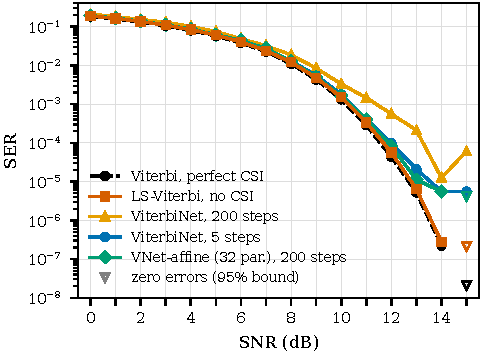
\includegraphics[width=\columnwidth]{ser_snr_letter.pdf}
\caption{SER vs.\ SNR. LS-Viterbi uses the same pilots and acceptance rule as the learned receivers, applied to its own decisions. Results are reported up to 14~dB; hollow triangles at 15~dB mark receivers with no errors (95\% upper bound).}
\label{fig:snr}
\end{figure}

\begin{figure}[t]
\centering
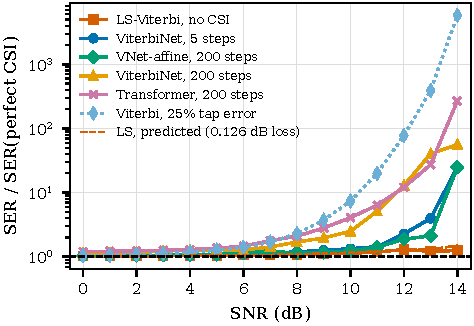
\includegraphics[width=\columnwidth]{gap_ratio.pdf}
\caption{SER relative to the perfect-CSI Viterbi detector. Dashed red: LS-Viterbi predicted by~\eqref{eq:loss}. At 14~dB the $K=5$, VNet-affine, and LS points rest on 4 bit errors each, clustered in one or two repetitions.}
\label{fig:gap}
\end{figure}

\begin{table}[t]
\centering
\caption{SER of the RS-decoded bits and online adaptation cost per accepted word (one CPU thread).}
\label{tab:main}
\setlength{\tabcolsep}{2pt}
\footnotesize
\begin{tabular}{@{}lrcccc r@{}}
\toprule
Receiver & Param. & 7 dB & 10 dB & 12 dB & 14 dB & Adapt.\\
\midrule
Viterbi, perfect CSI & -- & \sercsiseven & \sercsiten & \sercsitwelve & \sercsifourteen & --\\
Viterbi, 25\% CSI error & -- & \sercsitwentyfiveseven & \sercsitwentyfiveten & \sercsitwentyfivetwelve & \sercsitwentyfivefourteen & --\\
LS-Viterbi (no CSI) & 4 & \serlsseven & \serlsten & \serlstwelve & \serlsfourteen & LS solve\\
ViterbiNet, $K{=}200$ & 7,002 & \servnetseven & \servnetten & \servnettwelve & \servnetfourteen & 209 ms\\
ViterbiNet, $K{=}5$ & 7,002 & \servnetfiveseven & \servnetfiveten & \servnetfivetwelve & \servnetfivefourteen & 5.2 ms\\
VNet-affine, $K{=}200$ & 32 & \seraffineseven & \seraffineten & \seraffinetwelve & \seraffinefourteen & 105 ms\\
\bottomrule
\end{tabular}
\end{table}

\subsection{Online adaptation overfits}
Fig.~\ref{fig:steps} sweeps the number of adaptation steps $K$ at 7~dB with 25 offline minibatches. For the 7,002-parameter network the SER is lowest at $K=5$ ($0.0249$) and rises steadily to $0.0315$ at $K=200$: repeated steps on a single 136-sample word fit its noise. Without adaptation ($K=0$) the SER is $0.0340$, so adaptation is useful, but a few steps suffice. From 0 to 14~dB, $K=5$ has the lower point-estimate SER at every point (Fig.~\ref{fig:snr}; these two sweeps used independent draws) and needs 40 times fewer adaptation updates per accepted word (Table~\ref{tab:main}).

\begin{figure}[t]
\centering
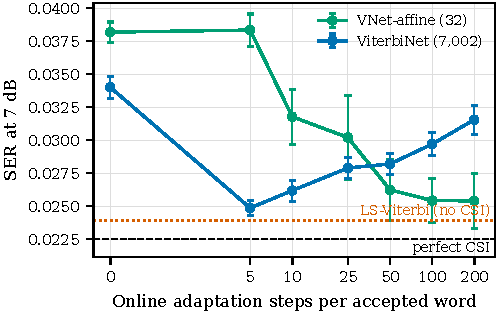
\includegraphics[width=\columnwidth]{online_steps.pdf}
\caption{SER at 7~dB vs.\ online adaptation steps per accepted word (25 offline minibatches; bars: 95\% confidence intervals over 20 repetitions).}
\label{fig:steps}
\end{figure}

\subsection{A 32-parameter metric and the latency budget}
The affine metric behaves differently: it starts from a generic offline solution and needs many steps to reach the frame's channel, reaching $0.0254$ at $K=100$--200, statistically tied with the tuned network (Fig.~\ref{fig:steps}). Over the SNR sweep it matches or beats ViterbiNet with $K=5$ from 8 to 13~dB (Fig.~\ref{fig:gap}). Widening the network does not help: in a sweep of 4 to 64 hidden units and two-layer variants at 7~dB, every larger model had a higher SER than the affine one at $K=200$ (point estimates; the smallest networks are within the confidence interval).

The parameter count matters little for latency. On one CPU thread of our implementation, the 136-step, 16-state trellis takes about 11~ms per word ($\approx$85~$\mu$s per symbol) for every receiver, while the network forward pass takes 0.05~ms (affine) to 0.14~ms (7,002 parameters). The cost that differs is adaptation: one step takes 0.5~ms for the affine metric and 1.0~ms for the network, so the affine metric at $K=200$ is not cheaper overall than the network at $K=5$. LS-Viterbi's adaptation is a $4\times4$ least-squares solve (0.02~ms). At 8~ksymbol/s a word lasts 17~ms; detection plus adaptation of one accepted word takes 11.4~ms for LS-Viterbi (the measured trellis time plus a separately timed 0.02~ms LS solve) and 16.8~ms for ViterbiNet with $K=5$ (1.4\% headroom), but 117~ms for VNet-affine and 220~ms for the default ViterbiNet. These are median component timings; RS decoding and gating are not included, so they do not establish a full receiver deadline. The trellis dominates the measured time only because it runs as an interpreted loop; in operation counts it costs $136\cdot2^{L+1}\approx4{,}400$ add-compare-selects per word, less than one forward pass of the network over the word ($\approx$$10^6$ multiply-accumulates), and LS re-estimation costs about $2{,}200$.

\section{Discussion and Conclusion}
For the studied linear Gaussian channel, the branch metric is determined by four taps. Estimating those taps from the same pilots and acceptance rule gives a receiver within about 3--30\% of the perfect-CSI SER, and none of the tested learned receivers has a lower point-estimate SER. This extends the original evaluation with an adaptive classical baseline; it does not contradict ViterbiNet's ability to learn a branch metric without explicit CSI. Our conclusion concerns this implementation and channel, and the meta-learned variants were not tested~\cite{raviv2021metaviterbinet,raviv2023online}. We recommend including this baseline and tuning the adaptation budget when assessing the benefit of learning.

The conclusions are limited to the setting studied: BPSK, one COST~2100 tap sequence, a linear Gaussian channel, and our implementation. Learned metrics can still help where the channel is nonlinear or the noise is non-Gaussian, where a four-tap model is wrong; testing those cases against a matched-information baseline is the natural next step.

\section*{Data Availability and AI-Use Statement}
Simulation code, raw results, and the scripts that generate every figure and table are available at \url{https://github.com/Gilzuk/viterbinet-revisited} (release \texttt{v1.0-submission}). An AI coding assistant (Claude, Anthropic) was used to write simulation and plotting code and to draft the manuscript; the author checked all code, results, and text.

\bibliographystyle{IEEEtran}
\bibliography{../refs}

\end{document}
